\section{Evaluation}
\label{sec:evaluation}

We first show the generated profile for the three applications. Then for each
application, We show how they adapt the behavior at runtime. Under a controlled
experiment, even with only transient network capacity drop, our system is able
to maintain an end-to-end delay for 10 seconds in the wide-area and accuracy
level above 80\%. Application-agnostic protocols creates significant backlogged
data (TCP for about 100 seconds) or unusable accuracy (UDP).

\subsection{Degradation Performance}
\label{sec:degr-perf}

\begin{figure*}
  \centering
  \begin{subfigure}[t]{0.30\textwidth}
    \centering
    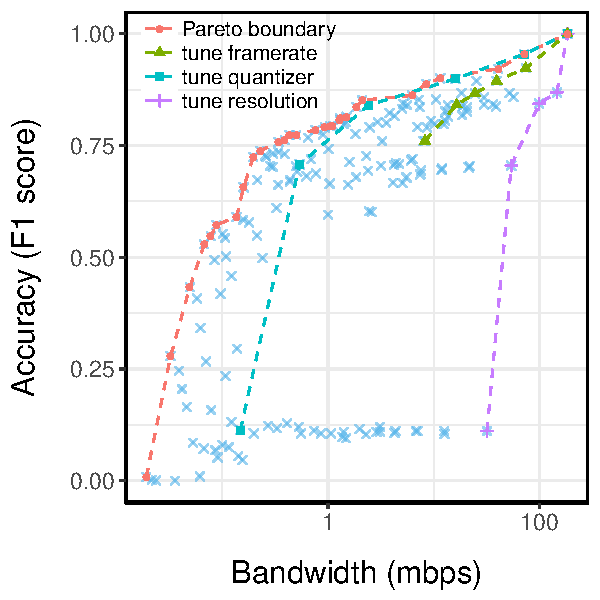
\includegraphics[width=\textwidth]{figures/ped-profile.pdf}
    \caption{Pedestrian Detection}
    \label{fig:pd-profile}
  \end{subfigure}
  ~
  \begin{subfigure}[t]{0.30\textwidth}
    \centering
    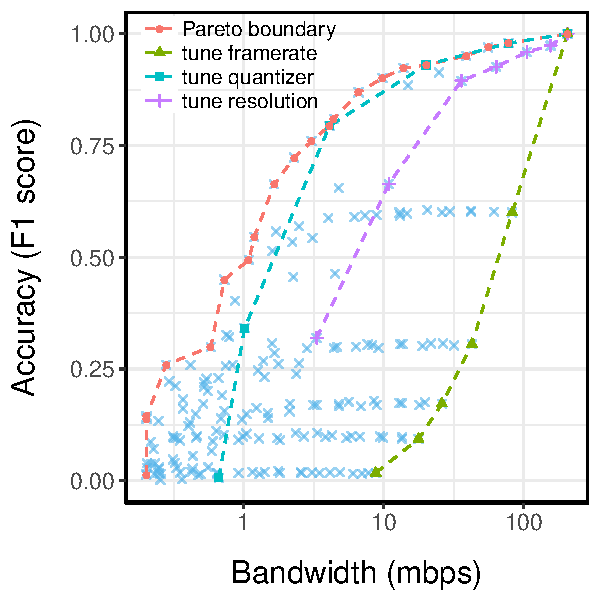
\includegraphics[width=\textwidth]{figures/darknet-profile.pdf}
    \caption{Augmented Reality}
    \label{fig:ar-profile}
  \end{subfigure}
  ~
  \begin{subfigure}[t]{0.30\textwidth}
    \centering
    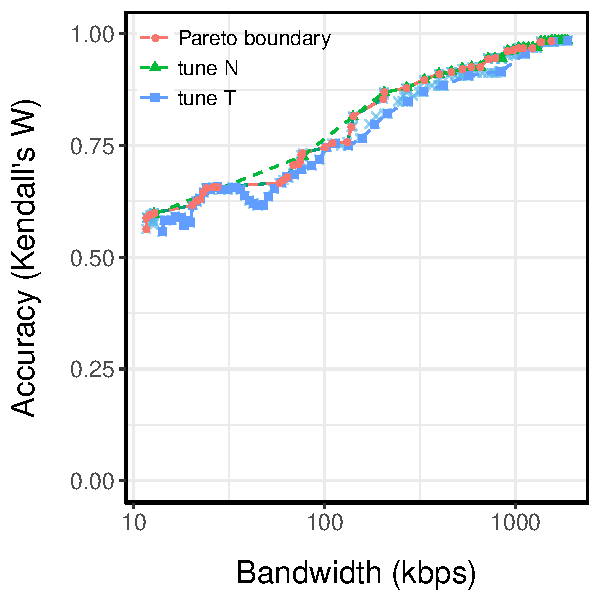
\includegraphics[width=\textwidth]{figures/log-profile.pdf}
    \caption{Top-k}
    \label{fig:tk-profile}
  \end{subfigure}
  \caption{Application profiles.}
  \label{fig:all-profiles}
\end{figure*}


We describe the dataset we used for offline profiling and interpret the
profiling results (\autoref{fig:all-profiles}) in turn.

\para{Pedestrian Detection:} We use MOT16 dataset~\cite{milan2016mot16} to
evaluate this application. Specifically we used MOT16-04 as the training
dataset. The video feeds capture a busy pedestrian street at night with an
elevated viewpoint. The original resolution is 1920x1080, with frame rate
30. The training data has 1050 frames in total, amounting 35-second monitoring.
On averge there are 45.3 people per frame.

There are three knobs in this application: resolution, frame rate and encoding
quality. To maintain the same 16:9 aspect ratio with the original 1920x1080
resolution, the first degradation only chooses common 16:9 resolutions:
1600x900, 1280x720, 960x540, 640x320. For the framerate, integer values are
chosen in favor of fraction values. The original frame rate is 30, and our
degradation explores 10, 5, 3, 2, 1. H.264 encoding quantizer has a range from 0
(lossless) to 51 (worst possible), and 18 is the visually
lossless~\cite{bellard2012ffmpeg}. In our experiment, we use 10, 20, 30, 40, 50
as degradation parameters.

The generated profile is shown in~\autoref{fig:pd-profile} with x-axis the
required bandwidth and the y-axis the accuracy (F1 score). Note the log scale on
the horizontal axis as raw uncompressed 8-bit RGB video streams are
prohibitively large: $1920 \times 1080 \times 30 \times 3 \times 8 = 1.5 $ Gbps.

Each point in the scatter plot represents one configuration that our offline
profiling has evaluated. Notice the vast spread in bandwidth requirement among
configurations with similar accuracy as well as the wide spread in accuracy
among configurations that consumes similar bandwidth.

We first show three lines in the case of only tuning one knob. Notice the
distinct behavior of the three lines. In this particular application, reducing
the resolution has the most penalty because the HOG detector has a minimal 128
pixels by 64 pixels window. The camera is deployed in a far-field context;
scaling down the image will quickly has an effect on the detection. Tuning frame
rate doesn't affect the accuracy too much. In fact, even with 1 FPS, the
accuracy is still relatively high. However, reducing frame rate doesn't bring
much bandwidth saving (as we have mentioned in \autoref{fig:h264}).  The most
effective way that reduces the bandwidth while preserving the accuracy is to
adjust the quantizer because it affects almost every pixel and creates smaller
P-frames.

The Pareto boundary, or \textit{profile}, is the most important curve. In the
begining it's close to the curve when only quantizer is tuned, quantizer has a
certain limit. A crisp image is prefered as many image processing algorithms are
looking for the edges while for human consumption, a smoother image is fine.

As the uncompressed video is not practical, we imposes a bandwidth cap before
the profile is used in runtime (only use optimal configurations that creates
video with less than 20mbps data rate).

\para{Augmented Reality:} We collected training set for this application
ourselves. It's a 23-second video clip with 1920x1080 resolution and 30 FPS
taken on a mobile phone. During the capture, we change the camera view in a slow
pace to emulate how a real user would look around. Because target objects are
relatively close while the camera is moving, we hypothesis for this training
set, the profile will be different from the previous application that reducing
frame rate will have a detrimental effect.

The generate profile is shown in \autoref{fig:ar-profile}. First, we see our
intuition backed up by measurements. Besides, the Pareto boundary also first
follows the video encoding knob, but optimal settings are achieved only when
multiple degradations are in effect.

\para{Top-K:} To evalute the top-k application, we generate synthetic dataset
based on real-world access logs (EDGAR log file dataset, the access log of
\url{https://sec.gov}). The original log contains CSV-format data extract from
Apache web server that records and stores user access
statistics~\cite{edgarlog}. The original log has only 500k access per hour; it's
rather small in comparison to today's CDN log. We condensed an hour-long data
into one second. After performing the local aggregation, the data size is
reduced from 500k entries per second to 50k key-value pairs (10x reduction).
Next we explore the space of degradation with respect to parameter N and T.  The
parameter N is from 100 to 15000; T from 0 to 500.

\autoref{fig:tk-profile} shows the generated profile. As we can see, most
configurations are very close to the pareto boundary. In the case when data skew
is more severe, we might see that T is more severe. Regardless, with our
automatic profiling tool, developers don't have to thoroughly understand the
complex relationship between bandwidth, accuracy and configuration.

\subsection{Runtime Performance}
\label{sec:runtime-performance}

\begin{figure*}
  \centering
  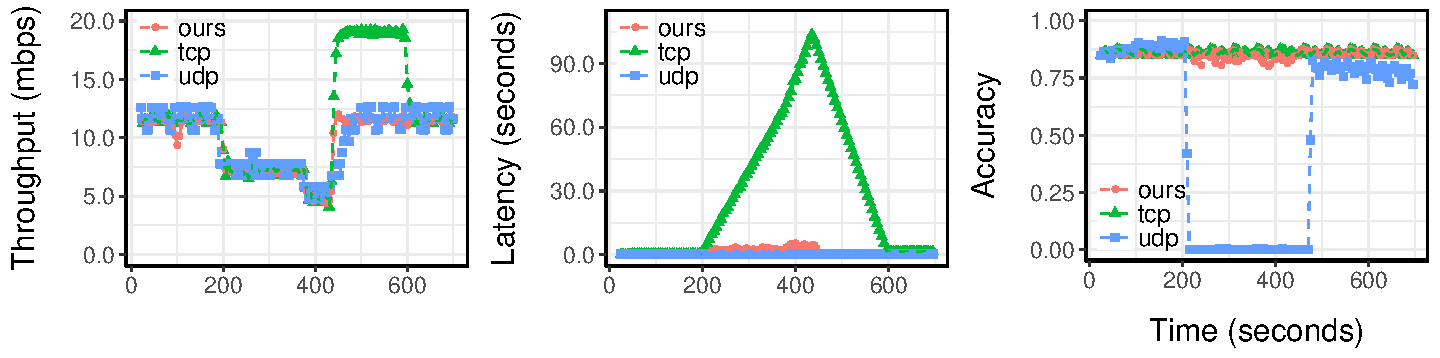
\includegraphics[width=0.95\textwidth]{figures/ped-runtime-horizontal.pdf}
  \caption{Runtime Adaptation of Pedestrian Detection}
  \label{fig:ped-runtime}
\end{figure*}

\begin{figure*}
  \centering
  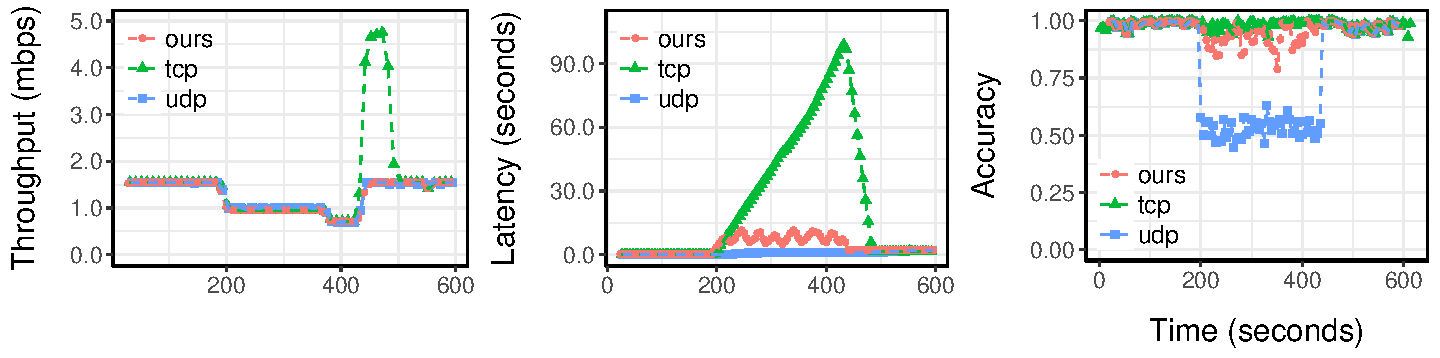
\includegraphics[width=0.95\textwidth]{figures/cdn-runtime-horizontal.pdf}
  \caption{Runtime Adaptation of Top-K}
  \label{fig:ped-runtime}
\end{figure*}

To evaluate the runtime behavior, we conduct controlled experiments using four
geo-distributed worker nodes from Amazon EC2 (t2.large instances) and an
aggregation server from our institute. For each experiment, worker nodes
transmit test data for about 10 mins. During each session, we use Linux
\texttt{tc} utility to adjust outgoing bandwidth to experiment with network
resource variation.

We compare our system with baseline systems that directly uses TCP and UDP. In
all three applications, the raw data streams are orders of magnitude
larger. While our system can adapt the rate, it could be unfair to baseline
solutions. We adjust the default degradation operation so that TCP and UDP would
work just fine when in normal cases; in this way, we make fair comparison. In
the case of UDP, shaping at the source doesn't emulate the packet loss behavior
with out-of-order delivery. We use \texttt{netem} to control packet loss rate to
match the desired shaping bandwidth.

In all three experiments, we see long delays in TCP. It increases linearly when
the traffic shaping started. When the bandwidth shaping stops, TCP quickly fills
the connection to recover. Depending on the queued size, the recovery could take
a few minutes or tens of seconds.

For UDP, the latency has been consistently small (mostly below 1 second) because
there is no queue building up. But when traffic shaping starts, the accuracy
drop is catastrophic.

Applications built with \sysname{} performs with a middle-ground behavior
between two extremes. We notice that our delay is still on the order of ten
seconds. The reason for the slow adaptation is three-folds: (1) our current
implementation only requests for bandwidth information when congestion is
detected, the delay of getting bandwidth estimation can be large in the case of
network capacity drop; (2) we perform the bandwidth in a conservative way with
smoothing to avoid sudden spikes. While more improvements are possible, the
current settings are satisfactory.

%%% Local Variables:
%%% mode: latex
%%% TeX-master: "sigcomm2017"
%%% End: